\documentclass[aspectratio=169]{beamer}
\usetheme{Pittsburgh}
\usecolortheme{spruce}
\usefonttheme{structurebold}
\beamertemplatenavigationsymbolsempty
\usepackage{graphicx}
\usepackage{tikz}

\title{Far Flung Forest Landscapes in the Anthropocene}
\subtitle{Structural analysis of China's embodied forest network}
\author{M.K. Lau (Ph.D.)}
\institute{Chinese Academy of Sciences and Harvard University}


\begin{document}

\begin{frame}
  \titlepage
\end{frame}


\begin{frame}
  \frametitle{Overview}

\tableofcontents

%% - Intro/Context
%%   - Forests are globally important
%%   - Anthropocence effects 
%%   - Global forest loss and gain and change
%% 	- Global greening = India(Agriculture) + China(Forests)
%% - Economics*Ecology = Landscape Extended Models
%% - Network Analysis of China's Greening
%%   - Global Scale
%%   - Local Scale
%% 	- Landscape = Chen 2019
%% 	- Resilience Analysis of China's Forest LE-MRIO
%% - Conclusions and Future Work
%% - Acknowledgements

\end{frame}


\section{Context}

\begin{frame}
  \frametitle{Forests are Important Globally}

  \begin{itemize}
  \item biodiversity
  \item water and nutrient cycling
  \item carbon storage
  \item resources(wood, food)
  \item culturally
  \end{itemize}

\end{frame}

\begin{frame}
  \frametitle{The Anthropocene}


  \begin{itemize}
  \item Humans = dominant global impact -> Anthropocene
  \item Global = Climate Change
  \item Indirect Effects Significant
  \end{itemize}


\end{frame}

\begin{frame}
  \frametitle{In the Anthropocene, Economy is Global Ecology}

  \begin{itemize}
  \item Economic trade data is a window into human impacts
  \item Brief history of IO and ENA analyses
  \item Global Trade Models
  \item Trade Networks MRIO = Sectors + Regions
  \item Environmental Extensions
  \item Forested Landscapes and Embodied Trade Networks
  \end{itemize}

\end{frame}

\begin{frame}
  \frametitle{Interactions/Trade = Complex Systems}

  \begin{itemize}
\item Indirect effecs and The far reach of the city
\item Complex systems = many players and indirect effects matter (surprising)

  \end{itemize}




\end{frame}



{ % all template changes are local to this group.
    \setbeamertemplate{navigation symbols}{}
    \begin{frame}<article:0>[plain]
        \begin{tikzpicture}[remember picture,overlay]
            \node[at=(current page.center)] {
                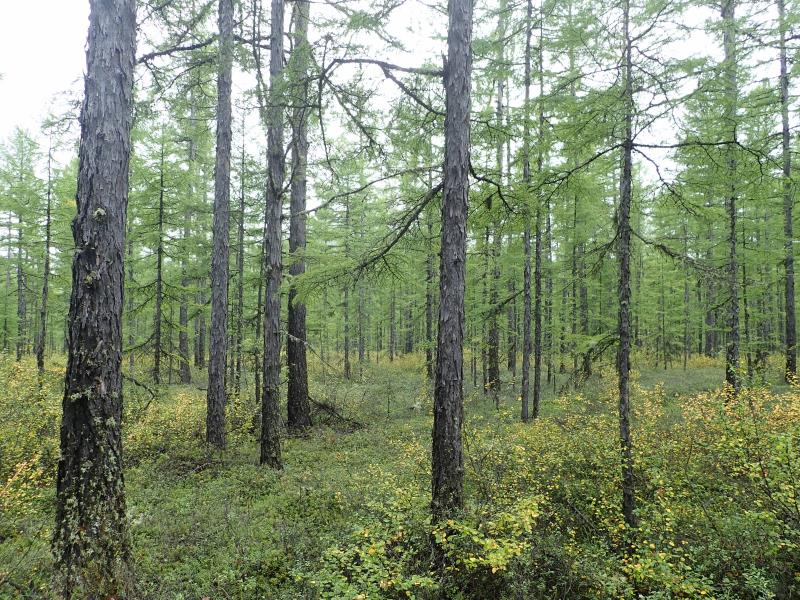
\includegraphics[keepaspectratio,
                                 height=\paperheight]{images/CNF/IMG_0194.JPG}
            };
        \end{tikzpicture}
     \end{frame}
}

{ % all template changes are local to this group.
    \setbeamertemplate{navigation symbols}{}
    \begin{frame}<article:0>[plain]
        \begin{tikzpicture}[remember picture,overlay]
            \node[at=(current page.center)] {
                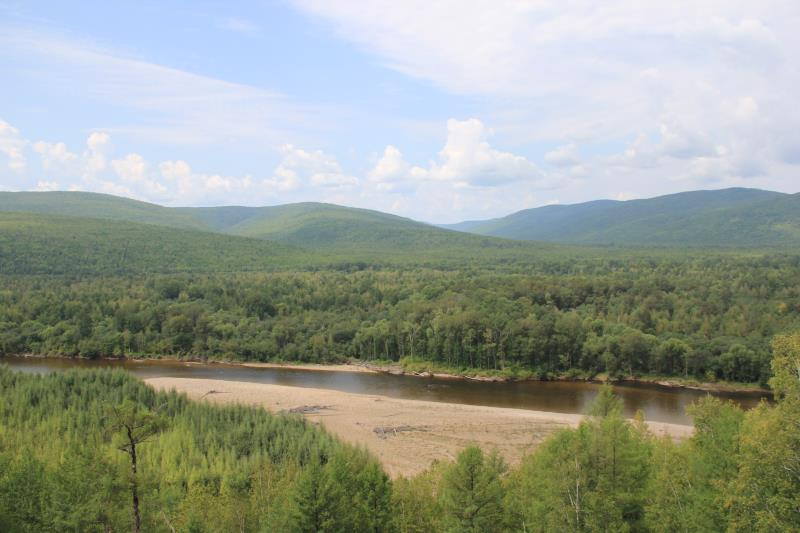
\includegraphics[keepaspectratio,
                                 height=\paperheight]{images/CNF/IMG_0199.JPG}
            };
        \end{tikzpicture}
     \end{frame}
}



\begin{frame}
  \frametitle{How do we study forests in this context?}


\end{frame}


\begin{frame}
  \frametitle{Background: Networks are Everywhere}


\begin{center}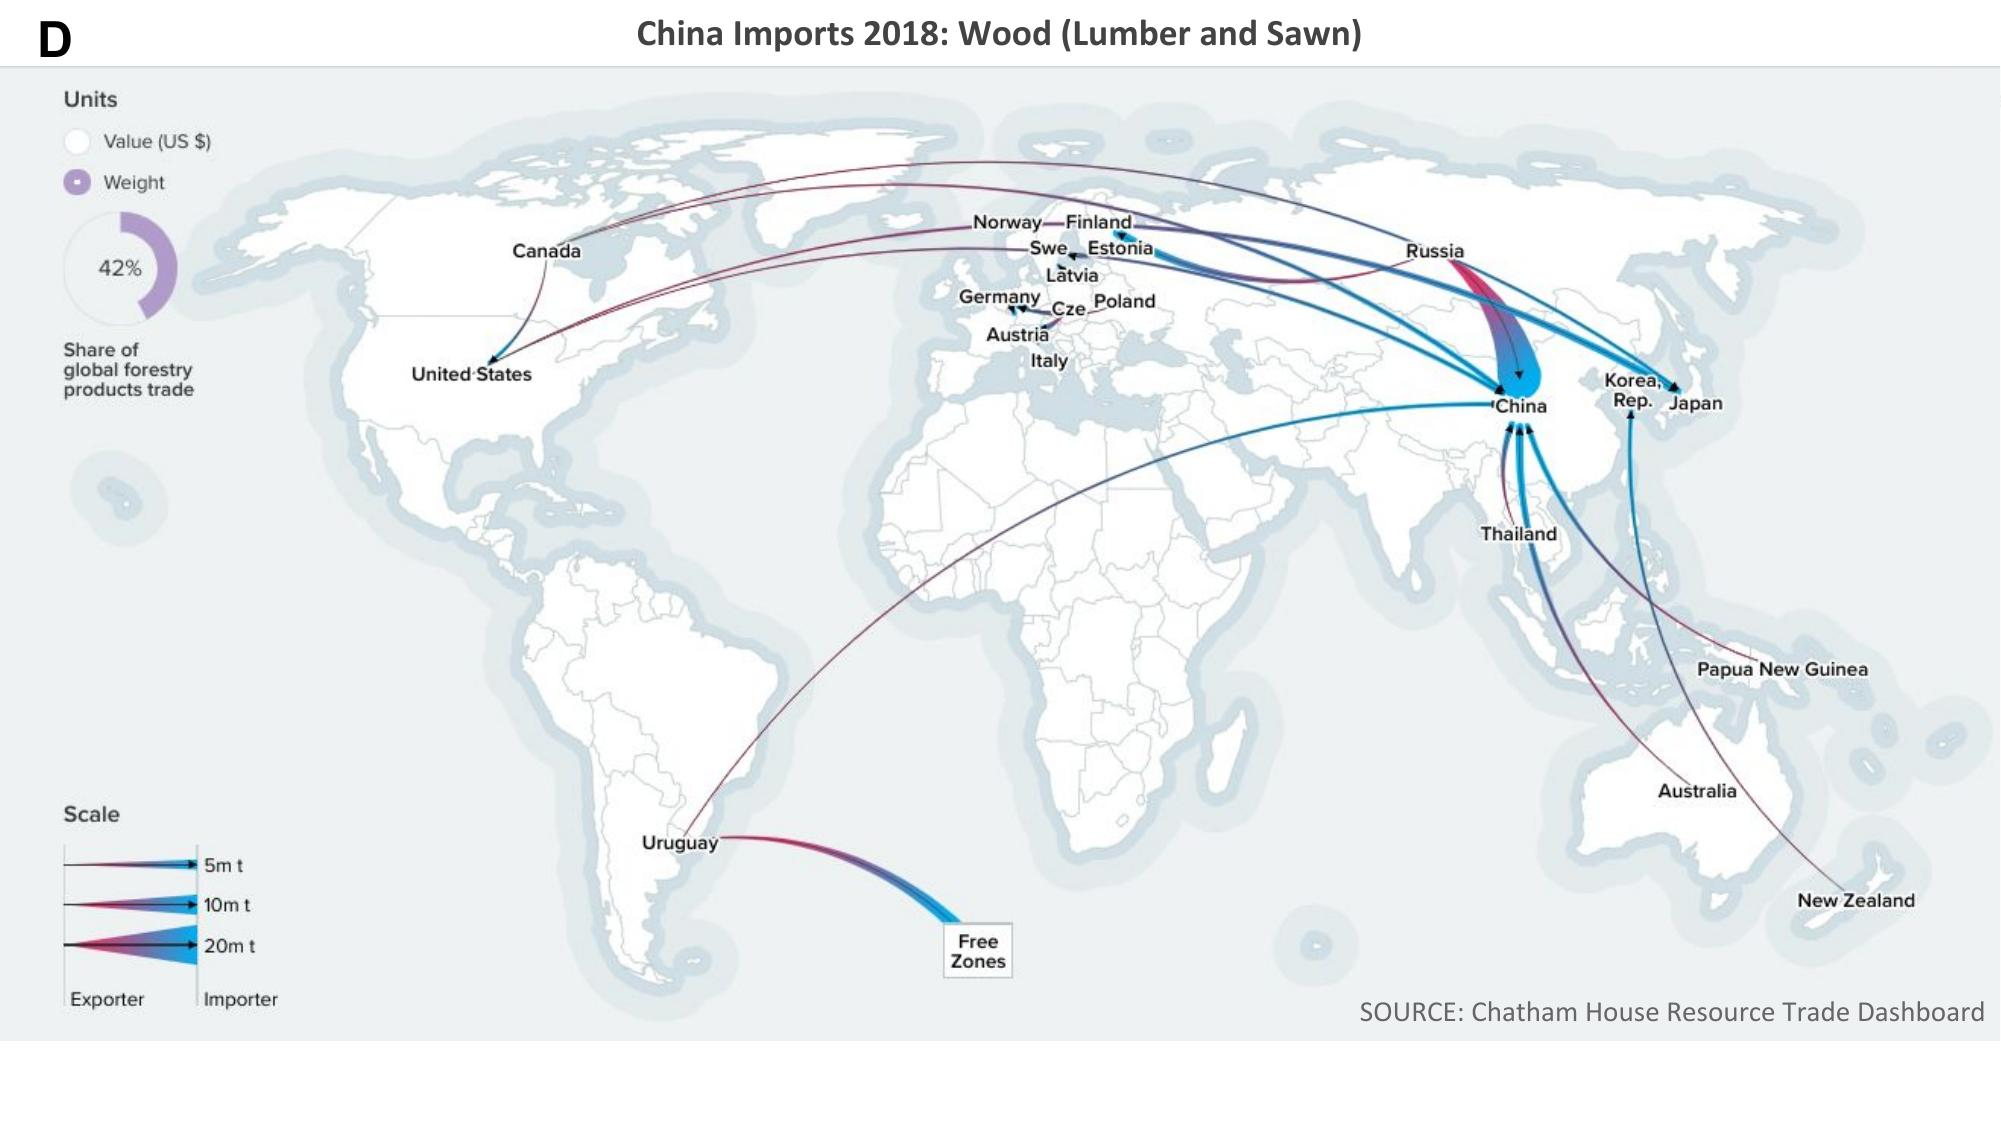
\includegraphics[width=0.5\linewidth]{images/resourcetrade_network} \end{center}

\end{frame}


\begin{frame}
  \frametitle{Background: Networks are Everywhere}

\begin{center}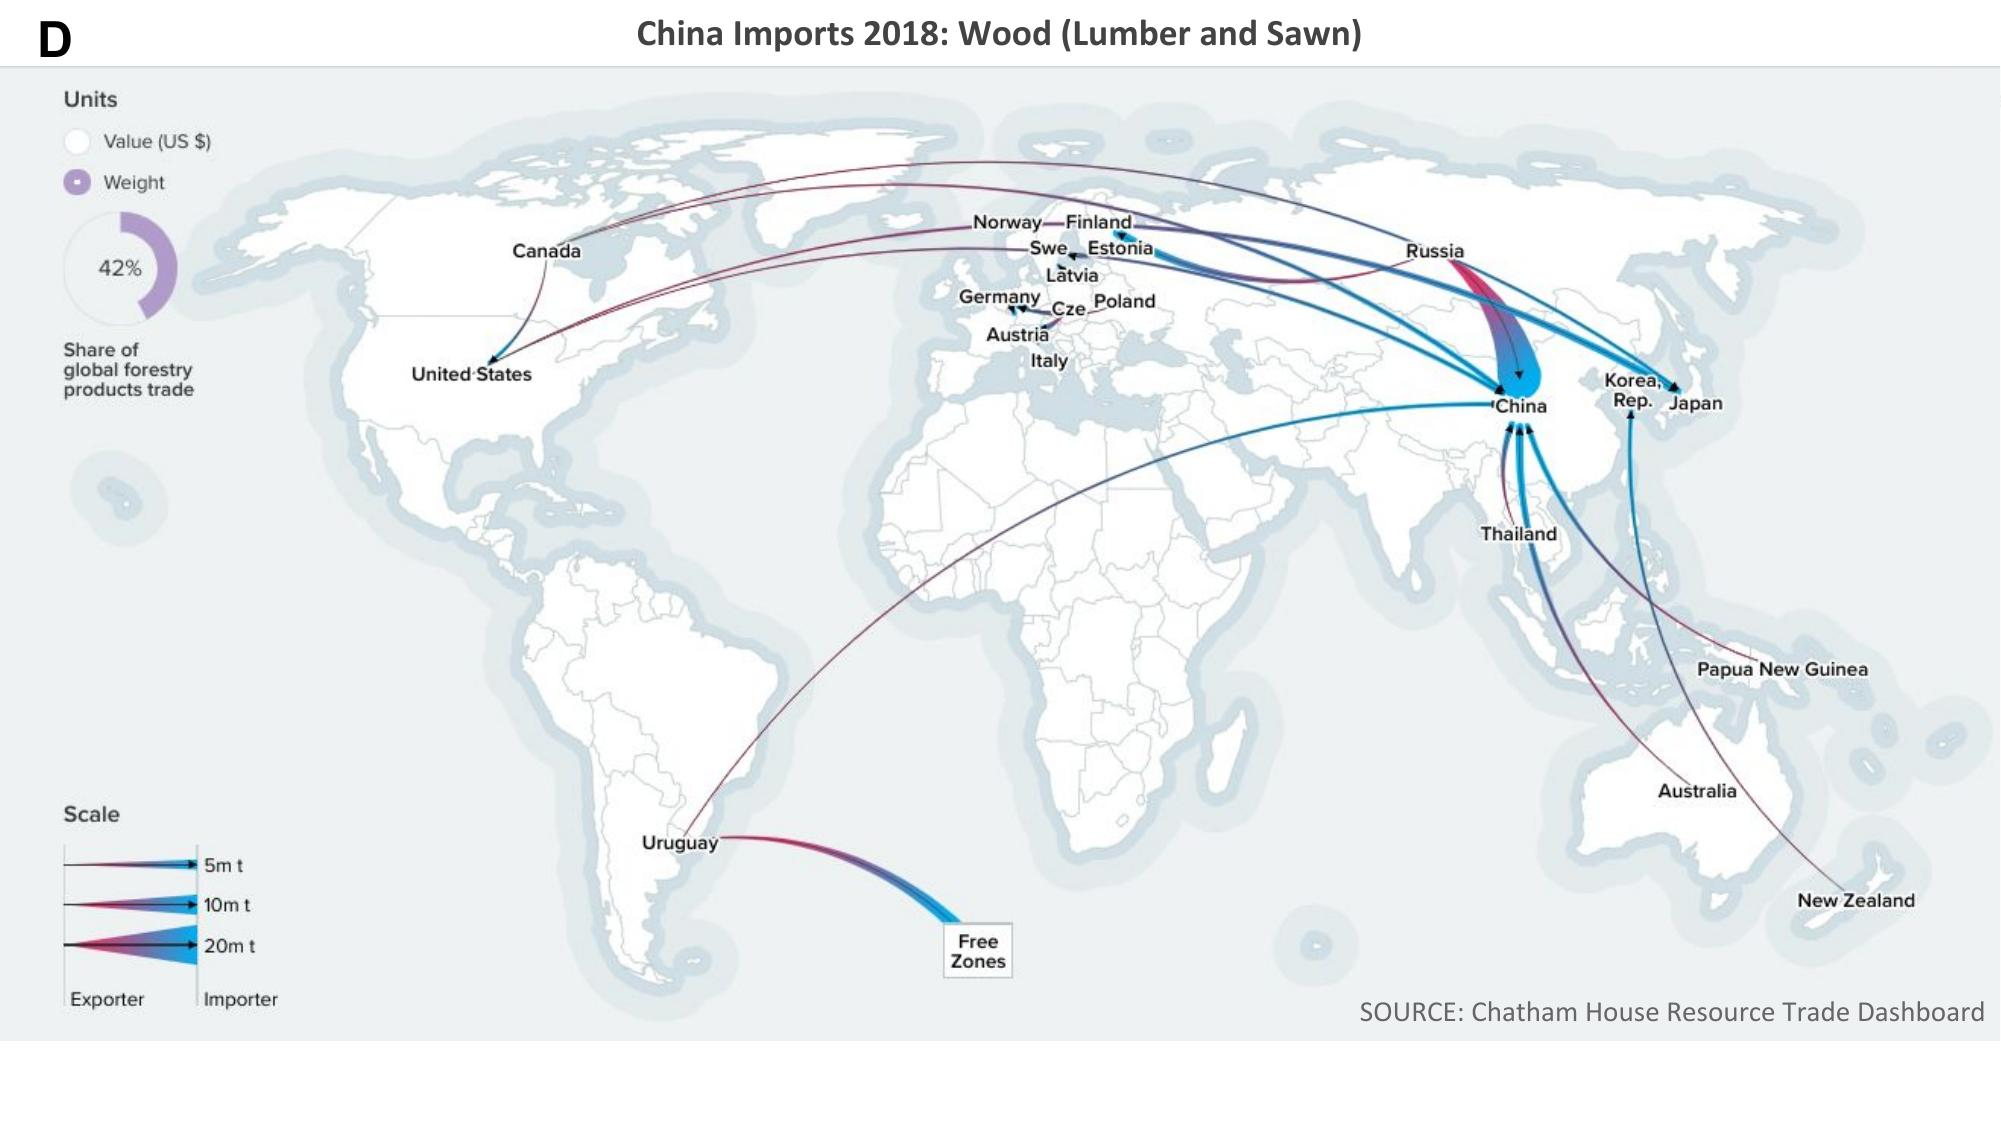
\includegraphics[width=0.5\linewidth]{images/resourcetrade_network} \end{center}


\end{frame}


\begin{frame}
  \frametitle{Background: Networks are Everywhere}

\begin{center}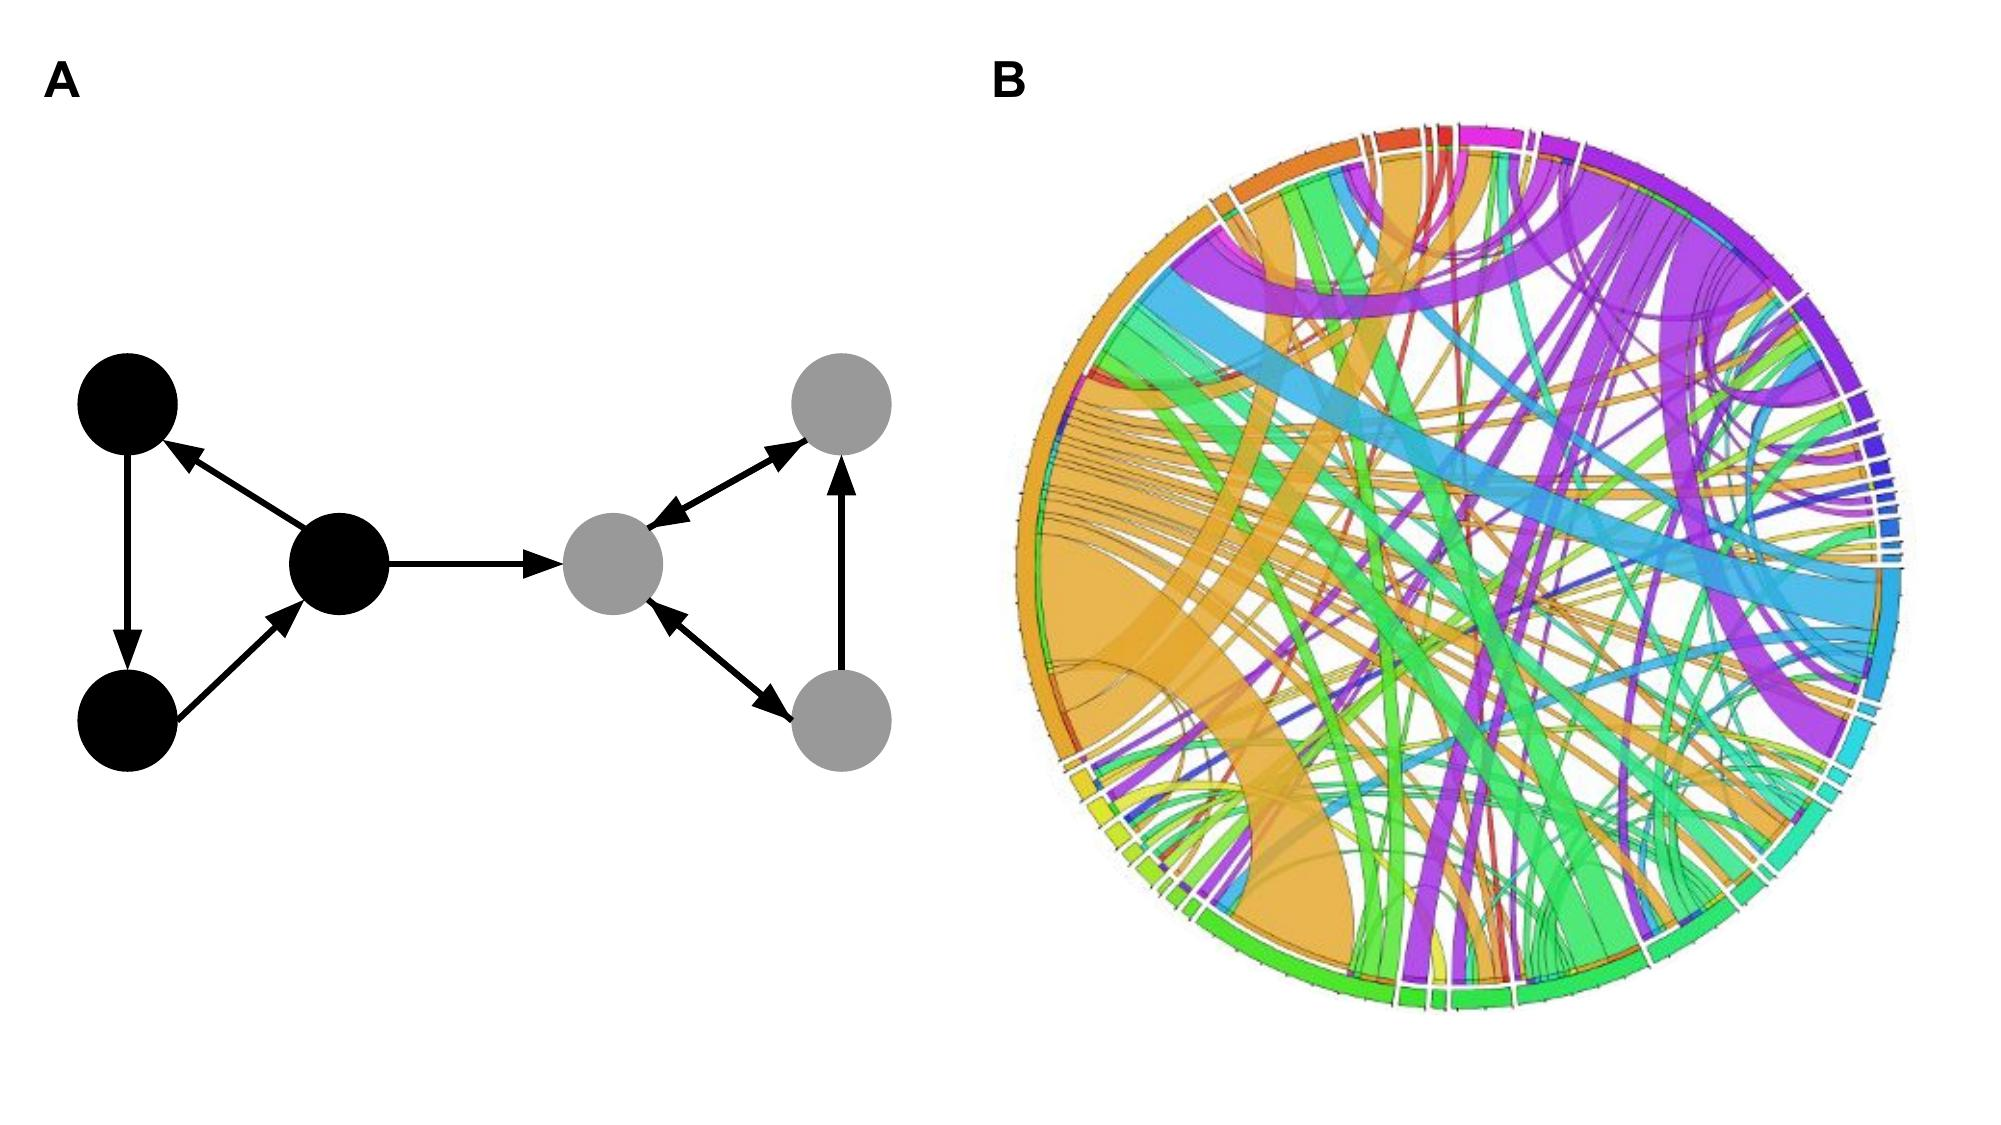
\includegraphics[width=0.5\linewidth]{images/example_network} \end{center}

\end{frame}

\begin{frame}
  \frametitle{Background: Ecological Network Analysis}

  \begin{itemize}
\item Ecological network theory provides predictions and metrics (Lau 2017)
\item Systems theory provides strategies for inteventions
\item ENA <- Odums, MacArthur, Ulanowicz, Patten,
\item SNA -> ecological networks (Watts and Strogatz, etc.)
\item Structure linked to function (Donella Meadows)
  \end{itemize}


\section{China's Forests}

\end{frame}

\begin{frame}
  \frametitle{Research: Why Chinese Forests?}

  \begin{itemize}
\item Work = Forest Land Embodied in Trade
  \end{itemize}

\end{frame}

\begin{frame}
  \frametitle{Global forest loss and gain and change}



\end{frame}

\begin{frame}
  \frametitle{Global greening}



\end{frame}

\begin{frame}
  \frametitle{Global greening = India(Agriculture) + China(Forests)}

  \begin{itemize}
  \item India is greening agriculturally
  \end{itemize}

\end{frame}

\begin{frame}
  \frametitle{Global greening = India(Agriculture) + China(Forests)}

  \begin{itemize}
  \item China is greening through reforestation 
  \end{itemize}

\end{frame}

\begin{frame}
  \frametitle{A Brief History of Forest Time in China}

  \begin{itemize}
  \item China is big and diverse (Tropical to Alpine/Boreal)
  \item Long history of human habitation in China
  \item Historically, two primary regions of forestry
  \item Forest conservation impacts harvest
  \item Flows within China and among countries globally important
  \end{itemize}

\end{frame}

\begin{frame}
  \frametitle{Research: Why Chinese Forests?}

\begin{center}\includegraphics[width=0.5\linewidth]{images/Forest_Cover_China.JPG} \end{center}

\end{frame}

\begin{frame}
  \frametitle{Research: Why Chinese Forests?}

\begin{center}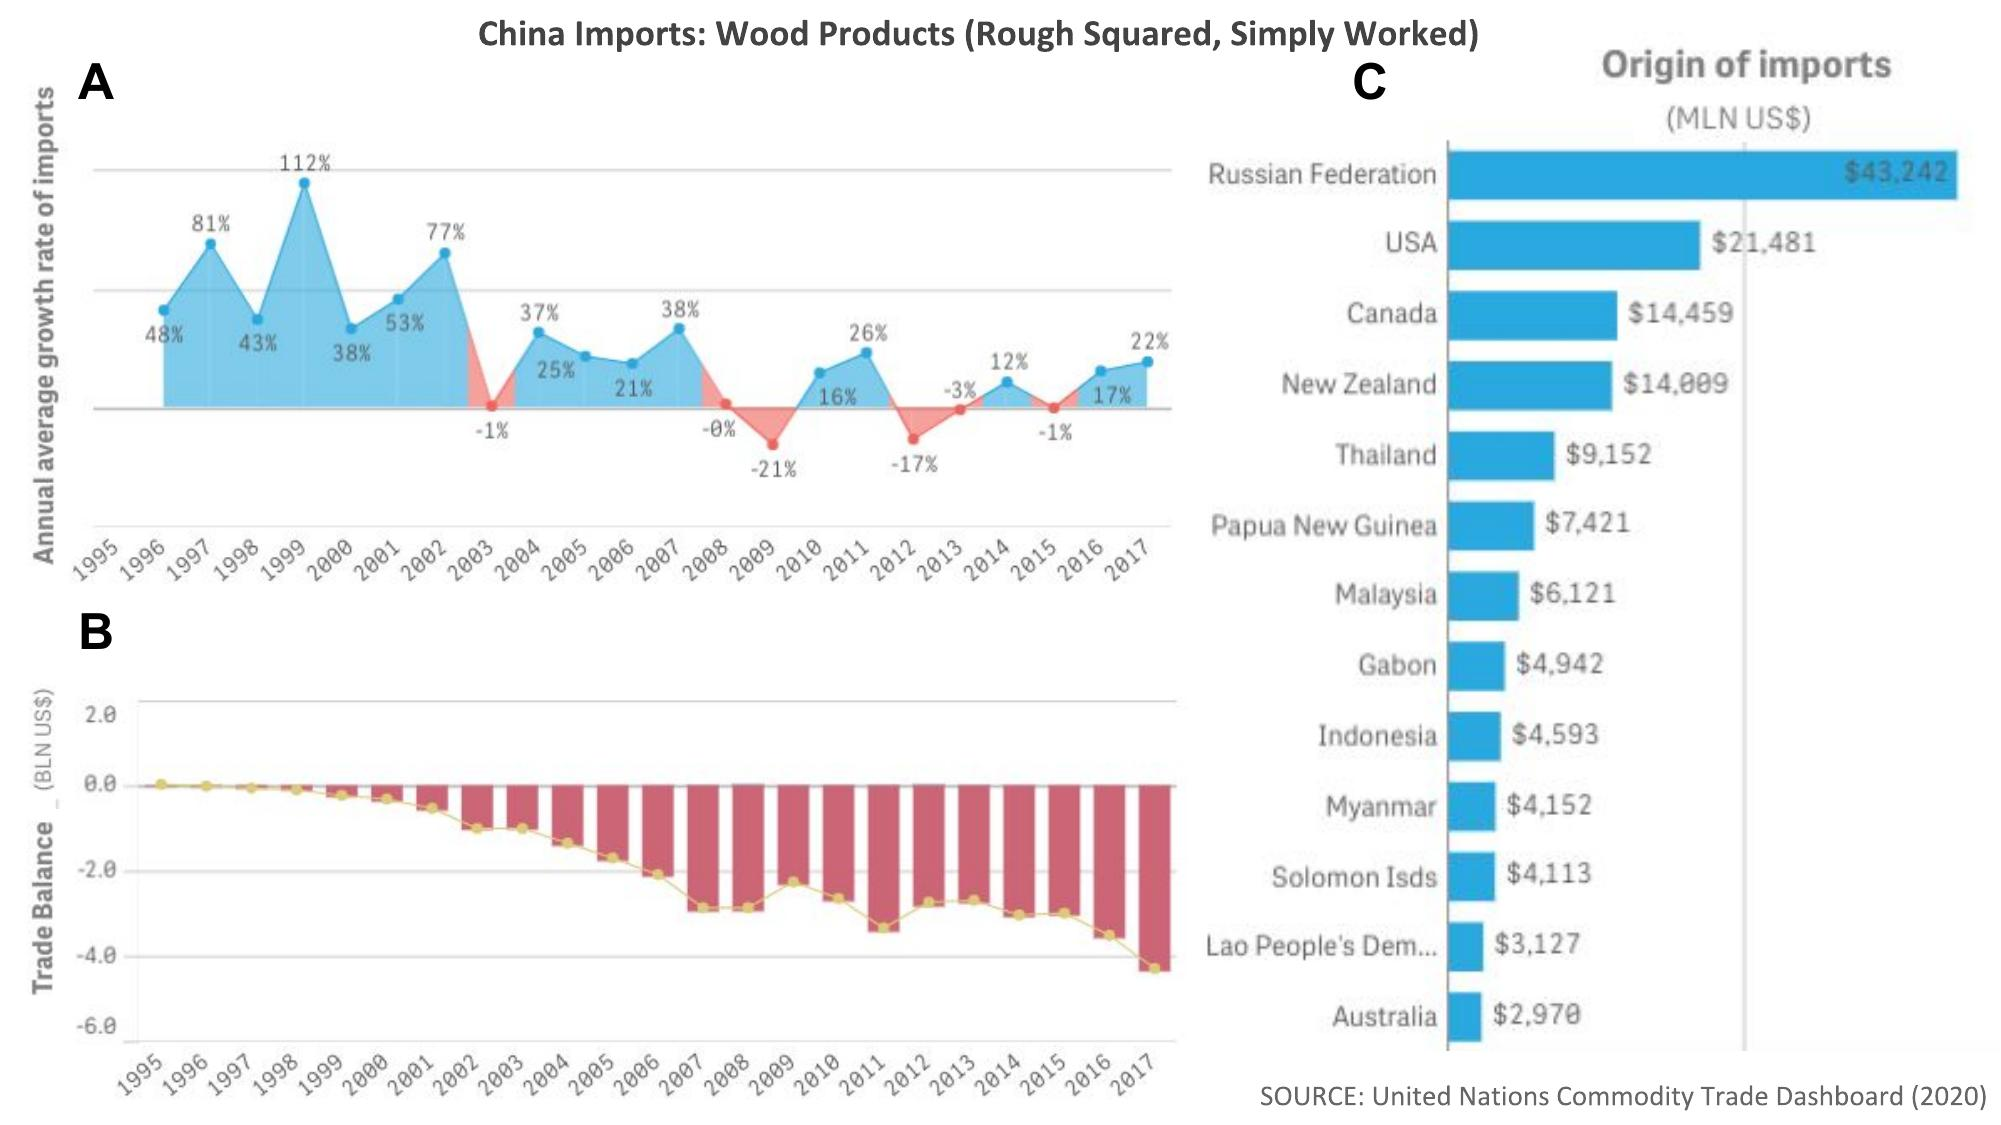
\includegraphics[width=0.5\linewidth]{images/comtrade_china_imports_wood.jpeg} \end{center}

\end{frame}

\begin{frame}
  \frametitle{Network Analysis of China's Greening}

  \begin{itemize}
  \item Global Scale
  \item Local Scale
  \item  - Landscape = Chen 2019
  \item  - Resilience Analysis of China's Forest LE-MRIO
  \end{itemize}

\end{frame}

\begin{frame}
  \frametitle{A little money moves a lot of forest. }

  \begin{itemize}
  \item Tian et al. 2019 showed that China consumes an equivalent amount
    of domestic cropland as forest land, on the order of 10$^6$ km$^2$.
  \item Looking at the domestic landuse productivity data for China,
    forests have the lowest monetary productivity.
  \item Thus, per unit monetary output a relatively larger amount of
    forest land is used.
  \end{itemize}

\begin{center}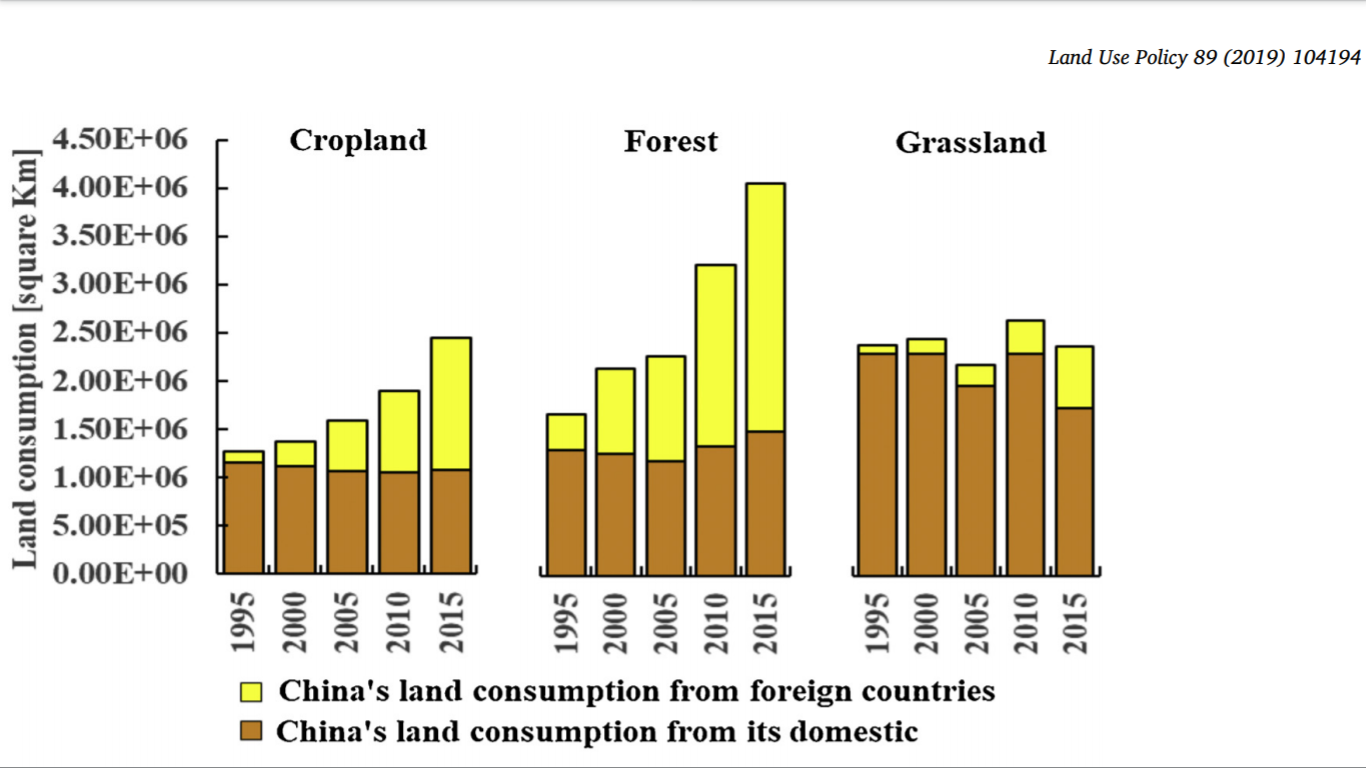
\includegraphics[width=0.5\linewidth]{images/Tian_2019_Fig1} \end{center}

\end{frame}

\begin{frame}{A little money moves a lot of forest.}

\begin{itemize}
\item
  Tian et al.~2019 showed that China consumes an equivalent amount of
  domestic cropland as forest land, on the order of 10\(^6\) km\(^2\).
\item
  Looking at the domestic landuse productivity data for China, forests
  have the lowest monetary productivity.
\item
  Thus, per unit monetary output a relatively larger amount of forest
  land is used.
\end{itemize}

\begin{center}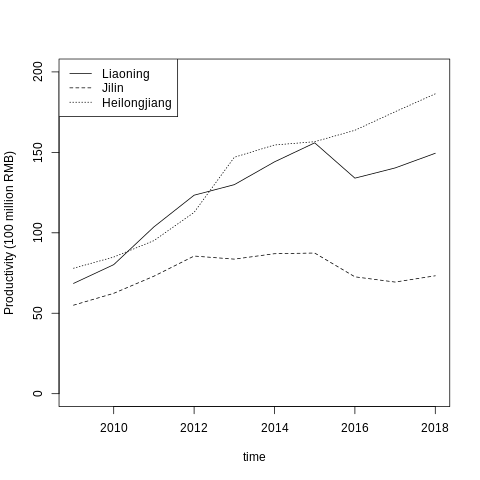
\includegraphics[width=0.5\linewidth]{images/prod_for_time_nec} \end{center}

\end{frame}

\begin{frame}{Global Landuse Trade and China}

\begin{center}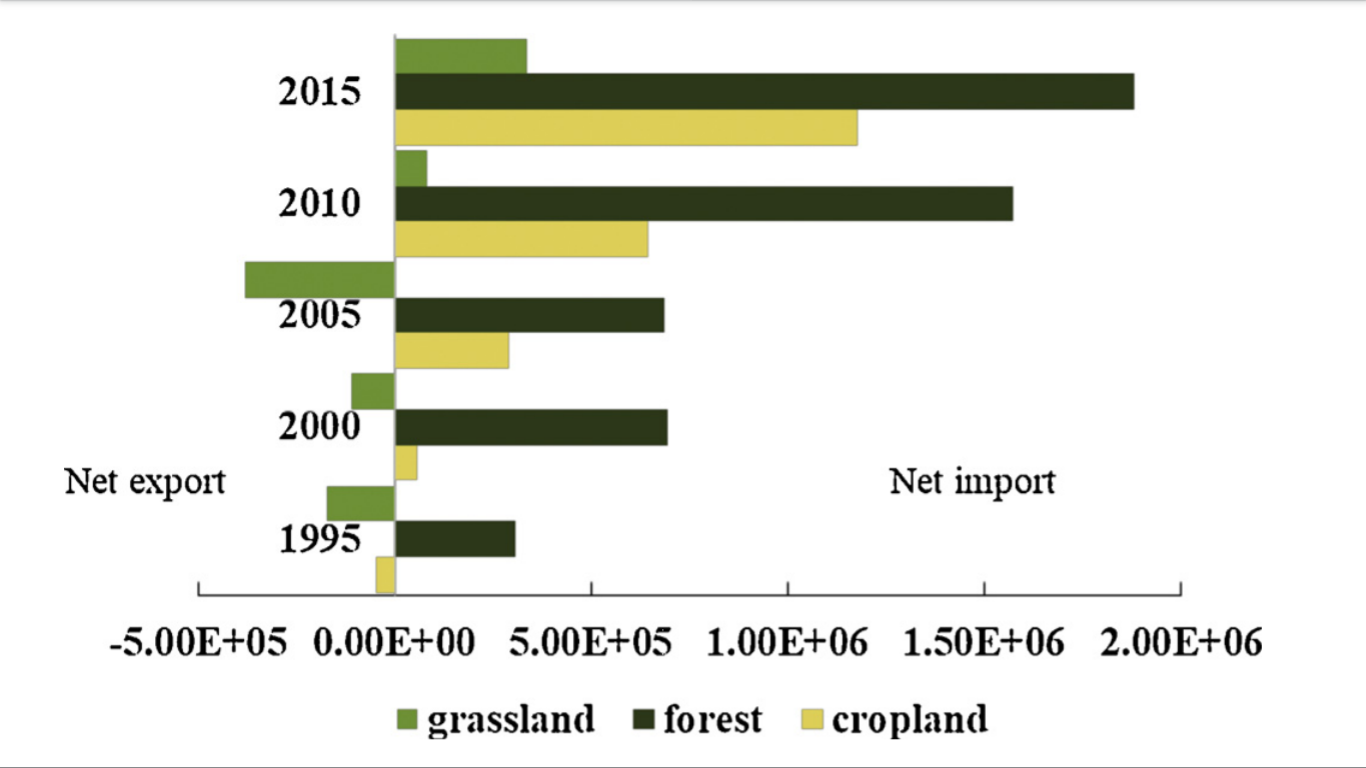
\includegraphics[width=0.5\linewidth]{images/Tian_2019_Fig2} \end{center}

\end{frame}

\begin{frame}{Global Landuse Trade and China}

\begin{center}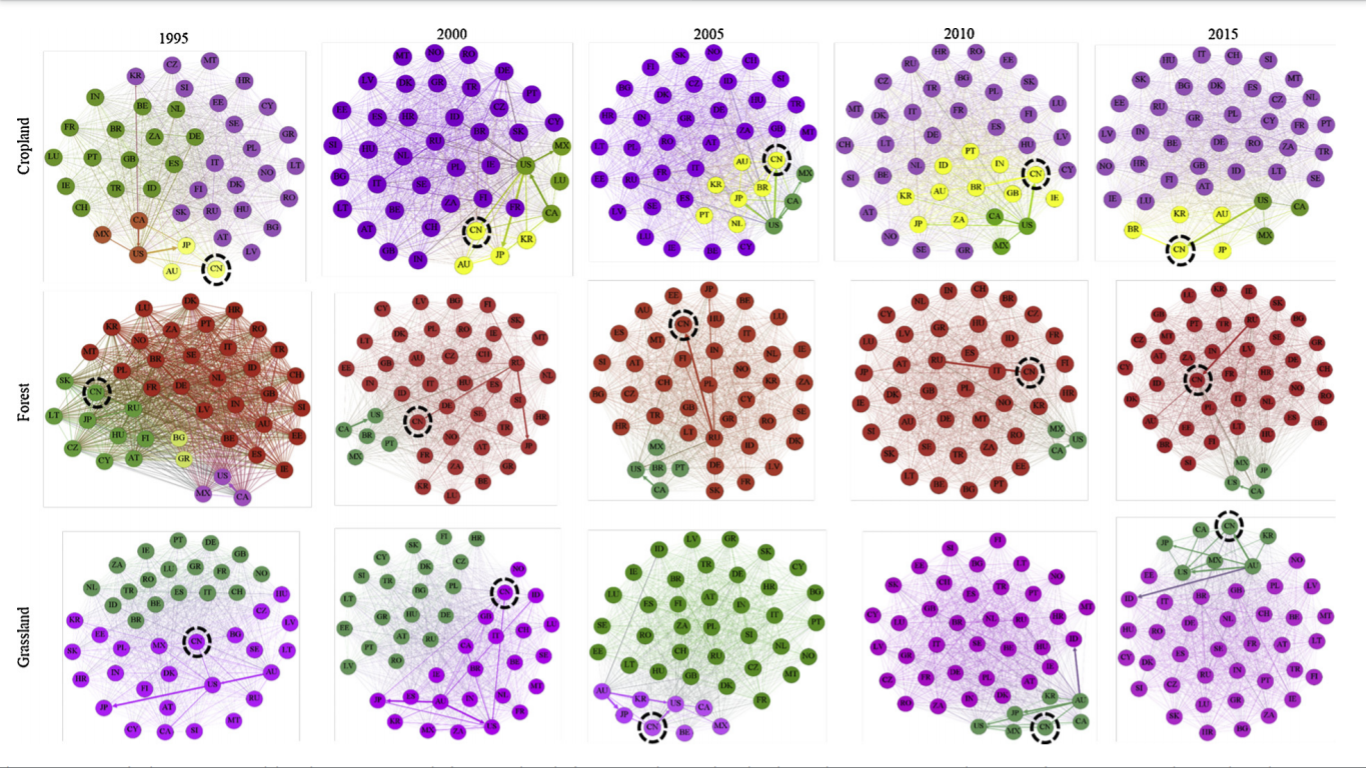
\includegraphics[width=0.5\linewidth]{images/Tian_2019_Fig3} \end{center}

\end{frame}

\begin{frame}{Background: Input-Output Models}

\begin{center}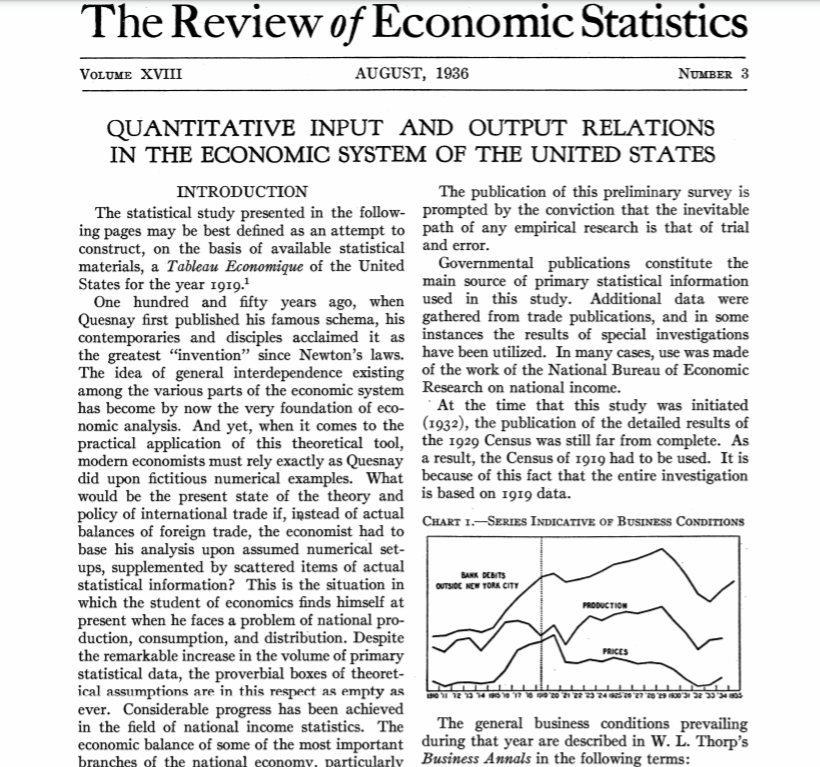
\includegraphics[width=0.5\linewidth]{images/leontief_1936} \end{center}

\end{frame}

\begin{frame}{Background: Input-Output Models}

\begin{itemize}
\item
  How do we quantify and manage systems?
\item
  Input-Output Analysis provides a modeling framework
\item
  Direct consumption
\item
  Trade occurs among sectors == Indirect consumption
\item
  IO and MRIO models
\item
  A new equation for a new era in science E = F(I-A)\^{}-1
\end{itemize}

\end{frame}

\begin{frame}{Background: Input-Output Models}

\begin{center}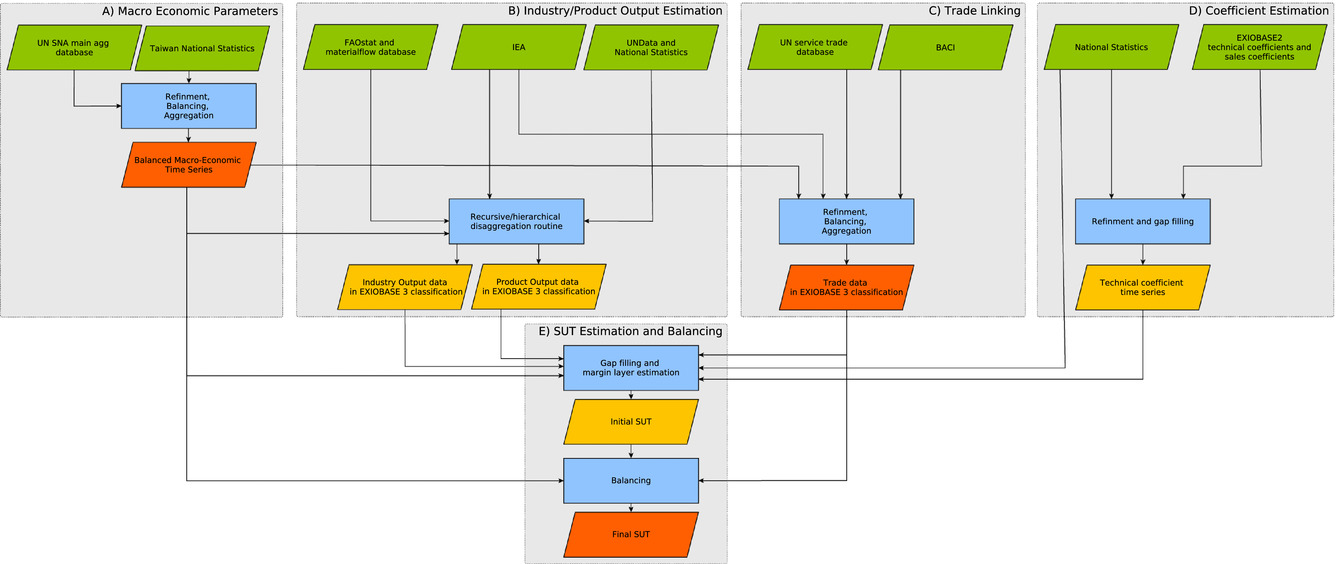
\includegraphics[width=0.5\linewidth]{images/exiobase3} \end{center}

\end{frame}

\begin{frame}{Background: Environmental Extension}

\begin{itemize}
\item
  Allows for indirect/consumption based accounting
\end{itemize}

\begin{center}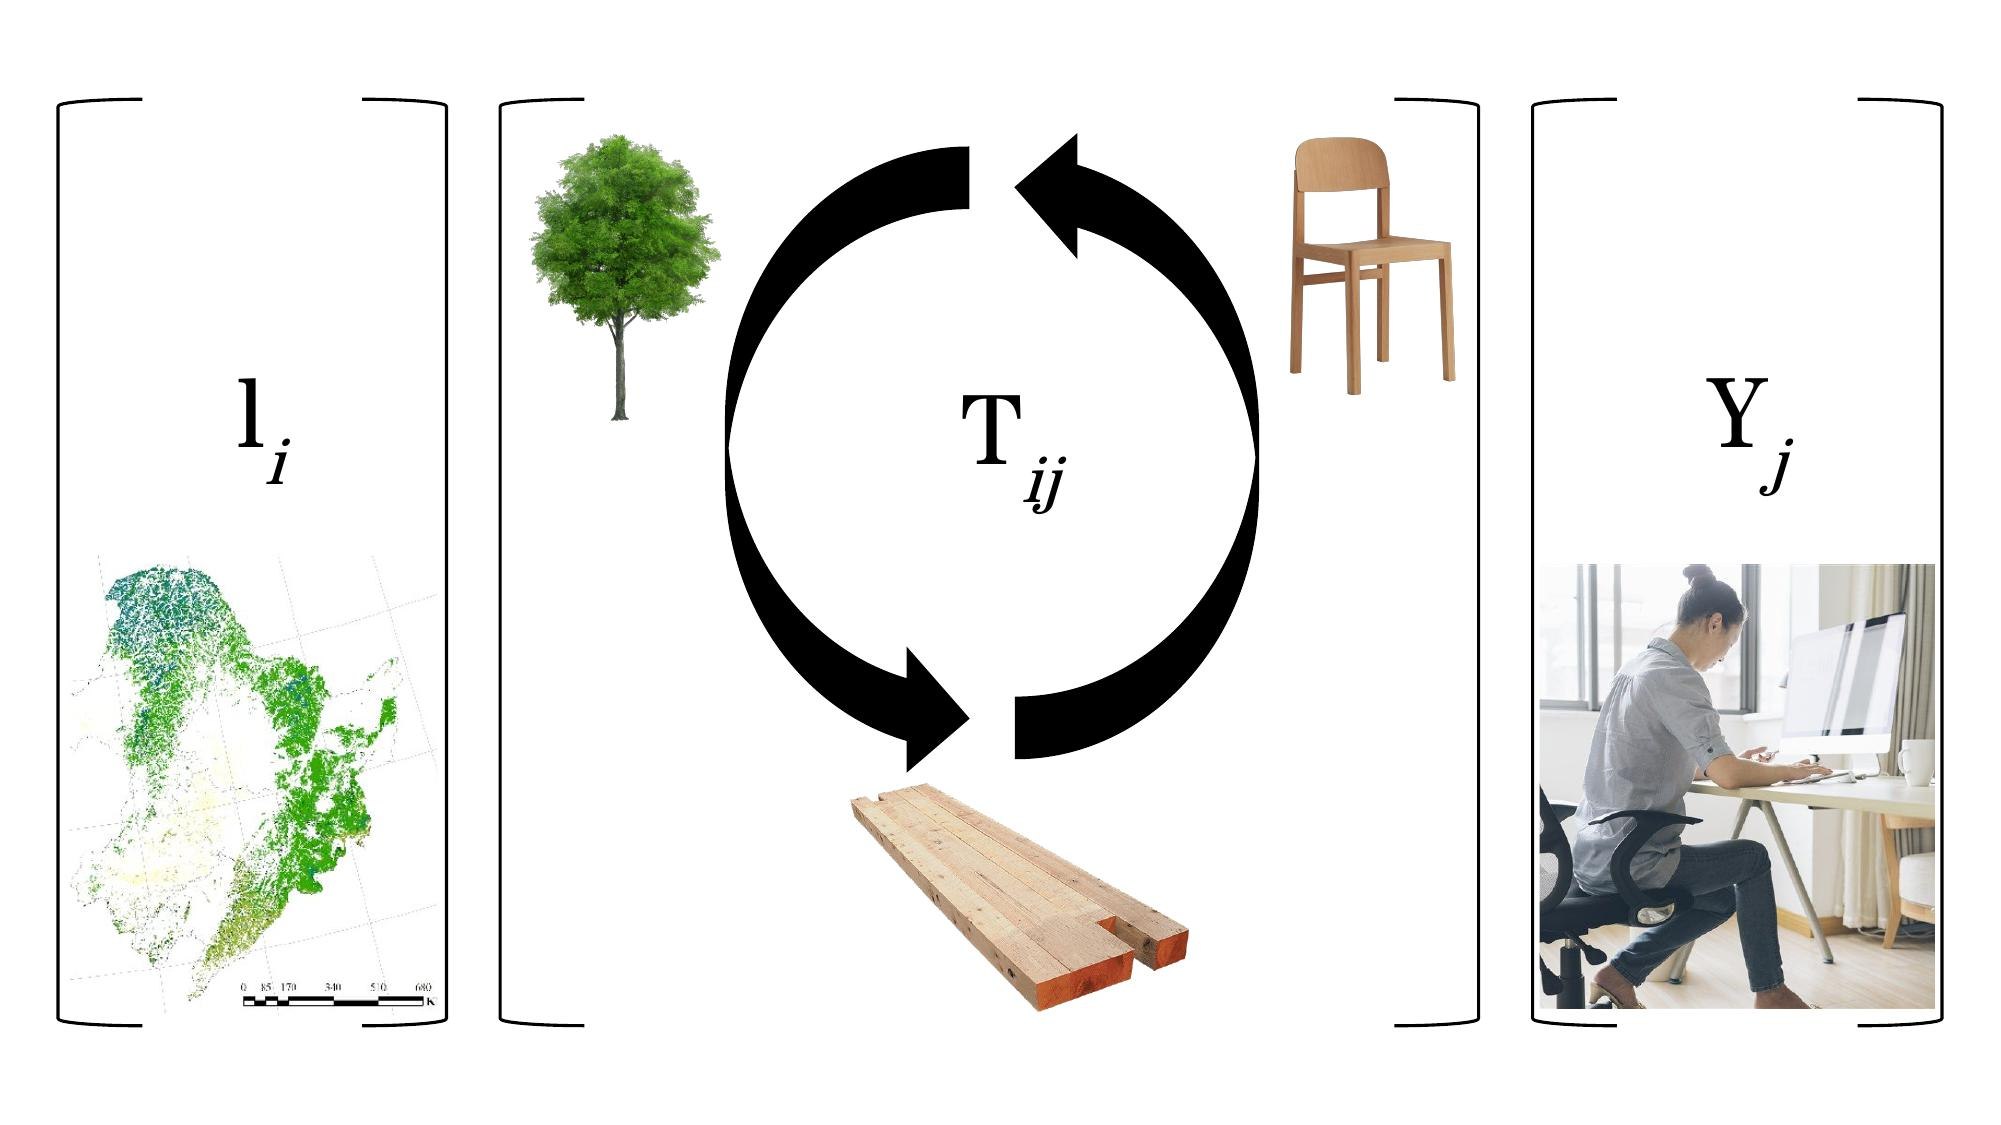
\includegraphics[width=0.5\linewidth]{images/lemrio} \end{center}

\end{frame}

\begin{frame}{Background: Environmental Extension}

\begin{center}\includegraphics[width=0.5\linewidth]{images/lemrio_equation} \end{center}

\end{frame}

\begin{frame}{wos\_mrio\_time.jpg}

\begin{center}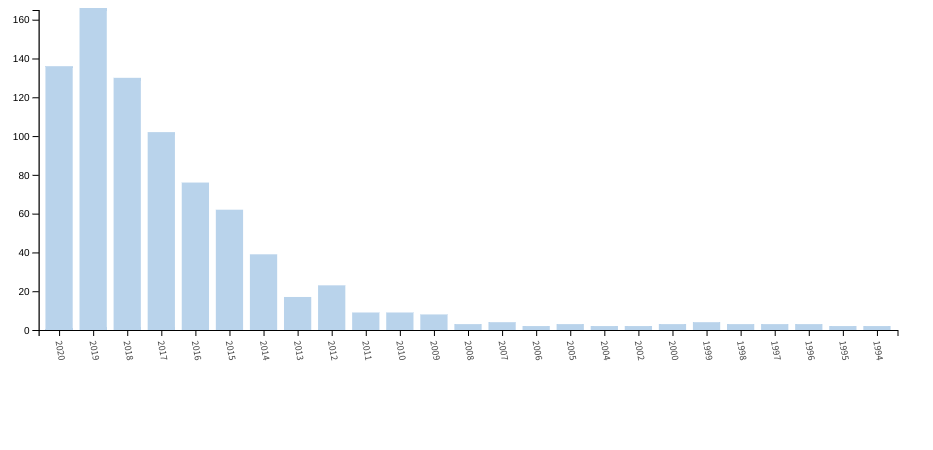
\includegraphics[width=0.5\linewidth]{images/wos_mrio_time} \end{center}

\end{frame}

\begin{frame}{wos\_mrio\_auth.jpg}

\begin{center}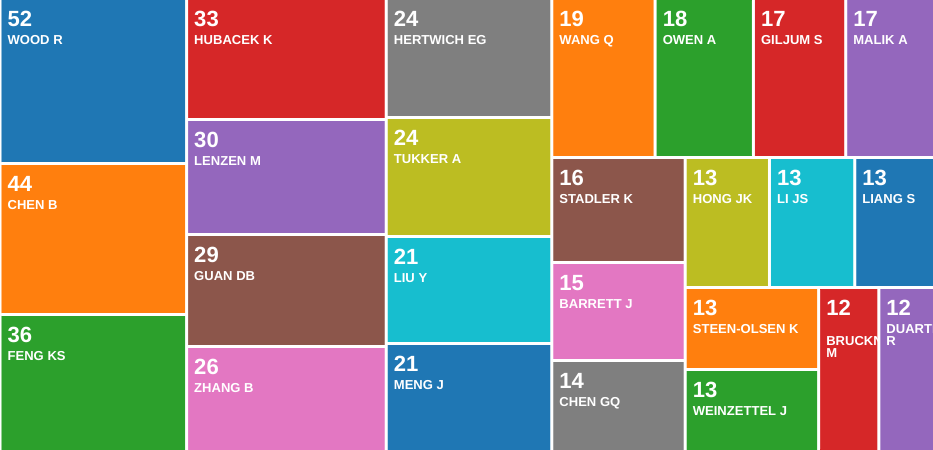
\includegraphics[width=0.5\linewidth]{images/wos_mrio_auth} \end{center}

\end{frame}

\begin{frame}{wos\_mrio\_funding.jp}

\begin{center}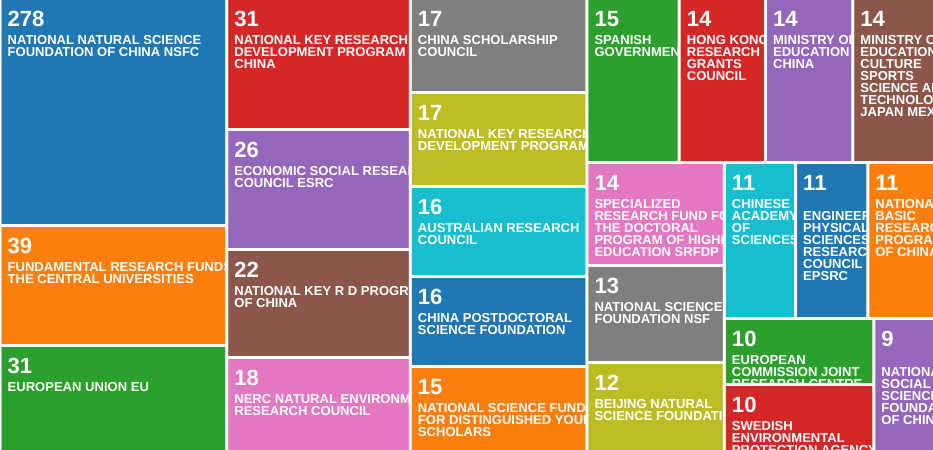
\includegraphics[width=0.5\linewidth]{images/wos_mrio_funding} \end{center}

\end{frame}

\begin{frame}{wos\_mrio\_field.jp}

\begin{center}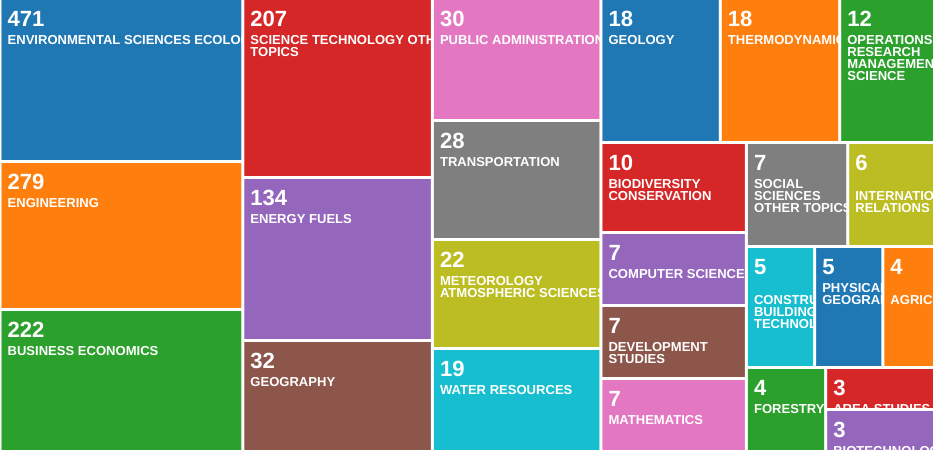
\includegraphics[width=0.5\linewidth]{images/wos_mrio_field} \end{center}

\end{frame}

\begin{frame}{wos\_mrio\_region.jpg}

\begin{center}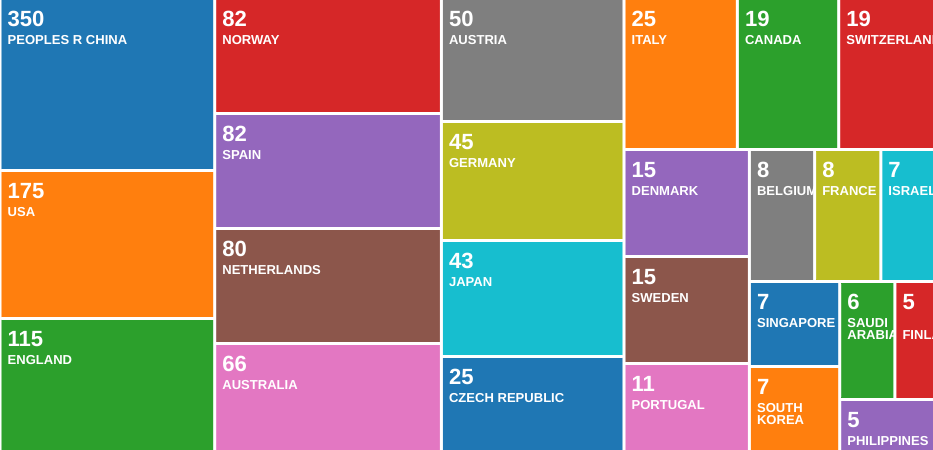
\includegraphics[width=0.5\linewidth]{images/wos_mrio_region} \end{center}

\end{frame}

\begin{frame}{Which metric?}

\begin{itemize}
\item
  Information
\end{itemize}

\end{frame}

\begin{frame}{Why information metrics?}

\begin{itemize}
\item
  Related to Shannon Information/Diversity index
\item
  \[H = -\sum_i^n p_i log(p_i)\]
\end{itemize}

\end{frame}

\begin{frame}{Methods: Model MRIO\(_{China}\)}

\begin{center}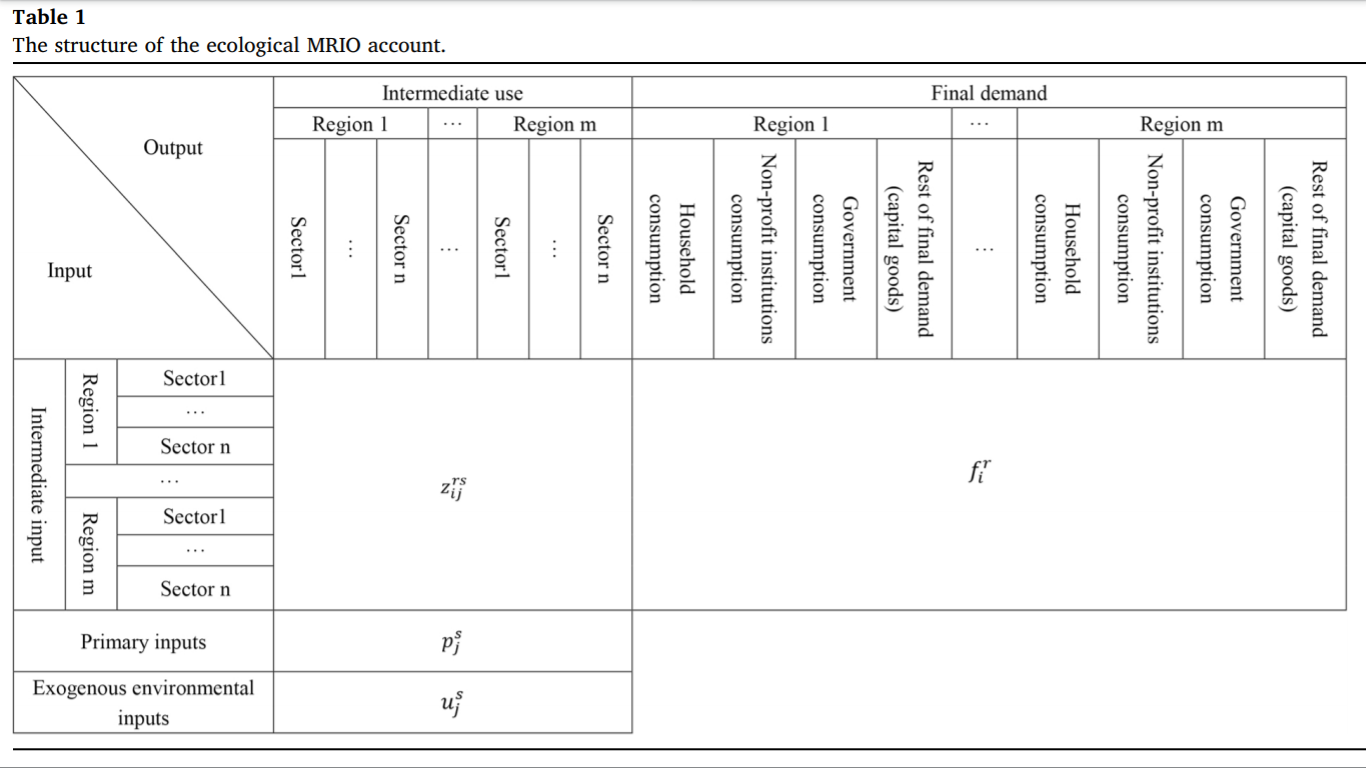
\includegraphics[width=0.5\linewidth]{images/Wu_2018_Table1} \end{center}

\end{frame}

\begin{frame}{Methods: Model MRIO\(_{China}\)}

\begin{center}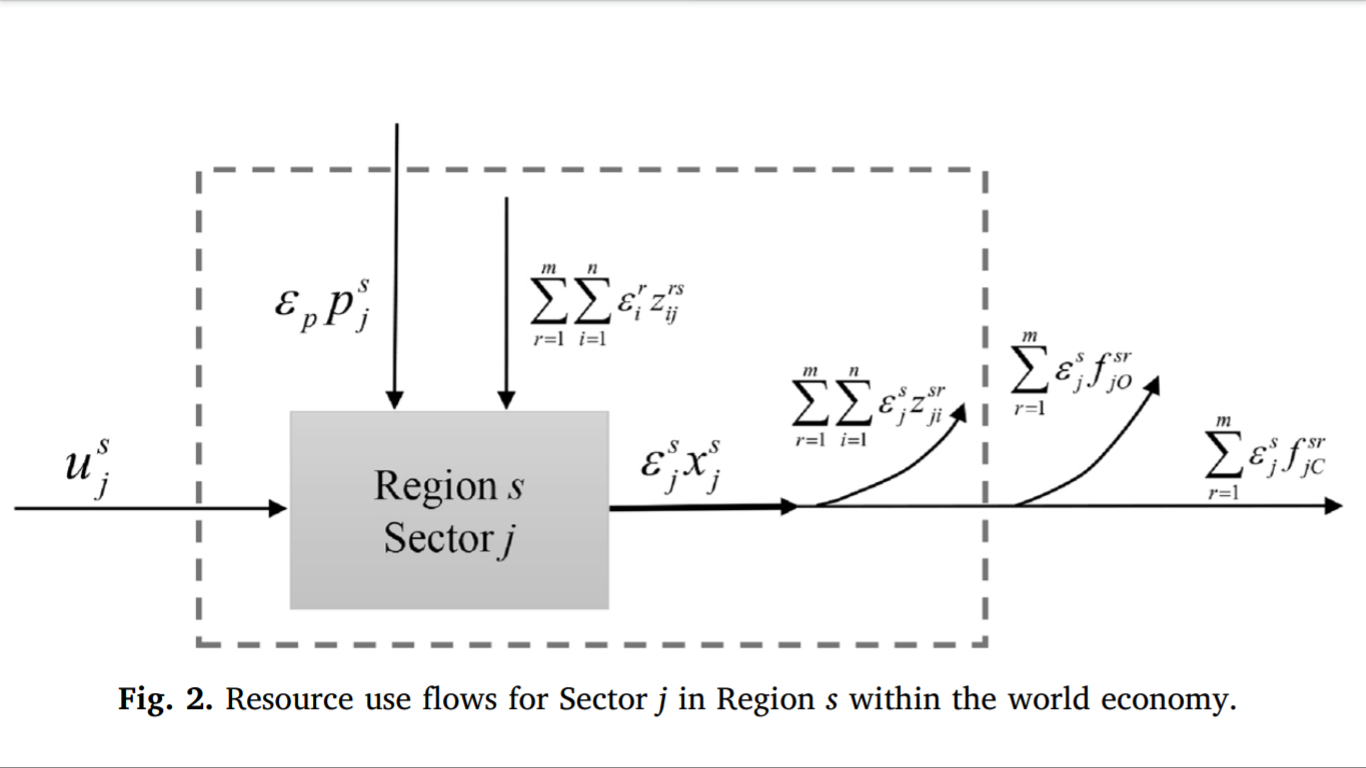
\includegraphics[width=0.5\linewidth]{images/Wu_2018_Fig2} \end{center}

\end{frame}

\begin{frame}{Methods: Environmentally Extended Model MRIO\(_{China}\)}

\begin{center}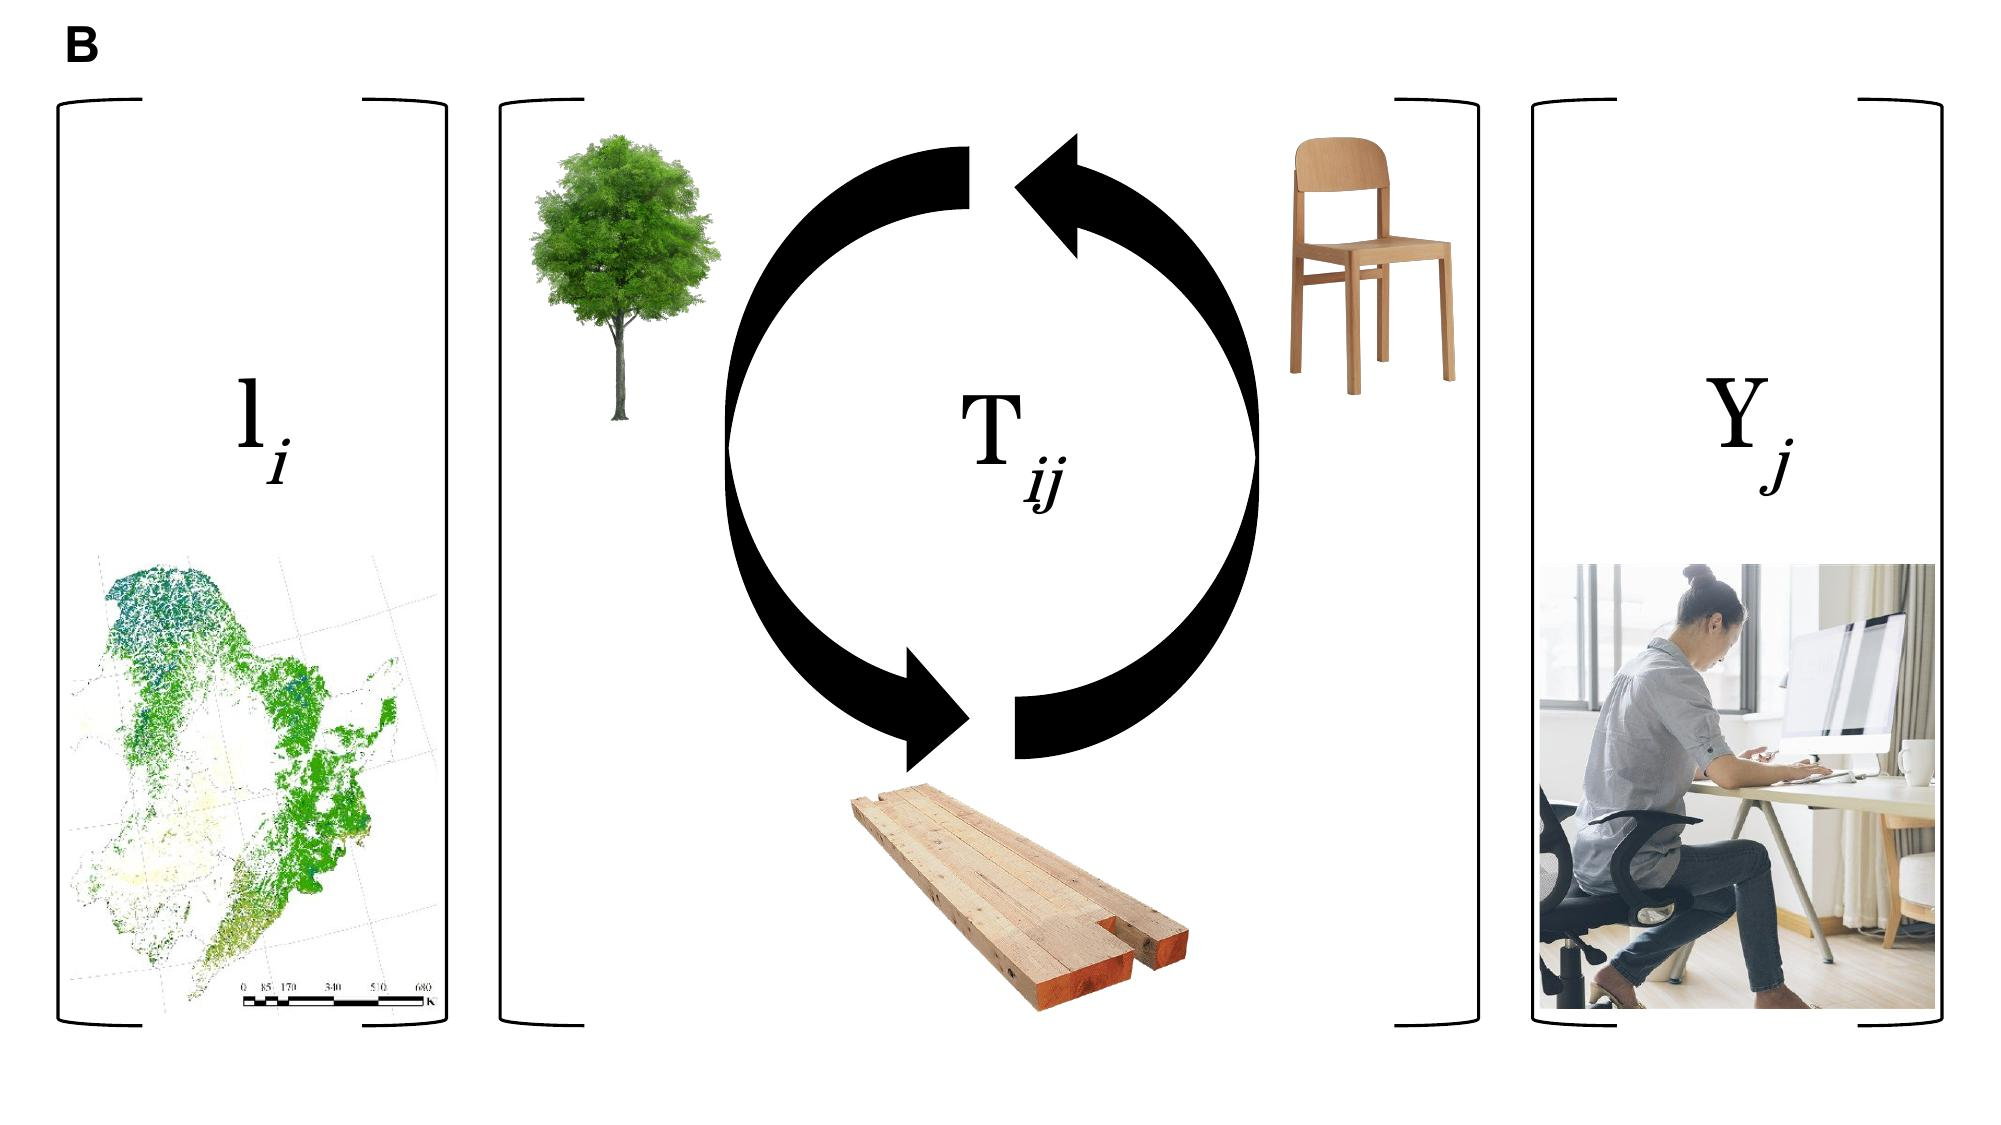
\includegraphics[width=0.5\linewidth]{images/china_eemrio} \end{center}

\end{frame}

\begin{frame}{Methods: Model Source}

\textbf{NEED TO ADD FIGURE WITH DATA FLOWS}

\emph{Maybe check the Mi 2018 supp mat}

\begin{center}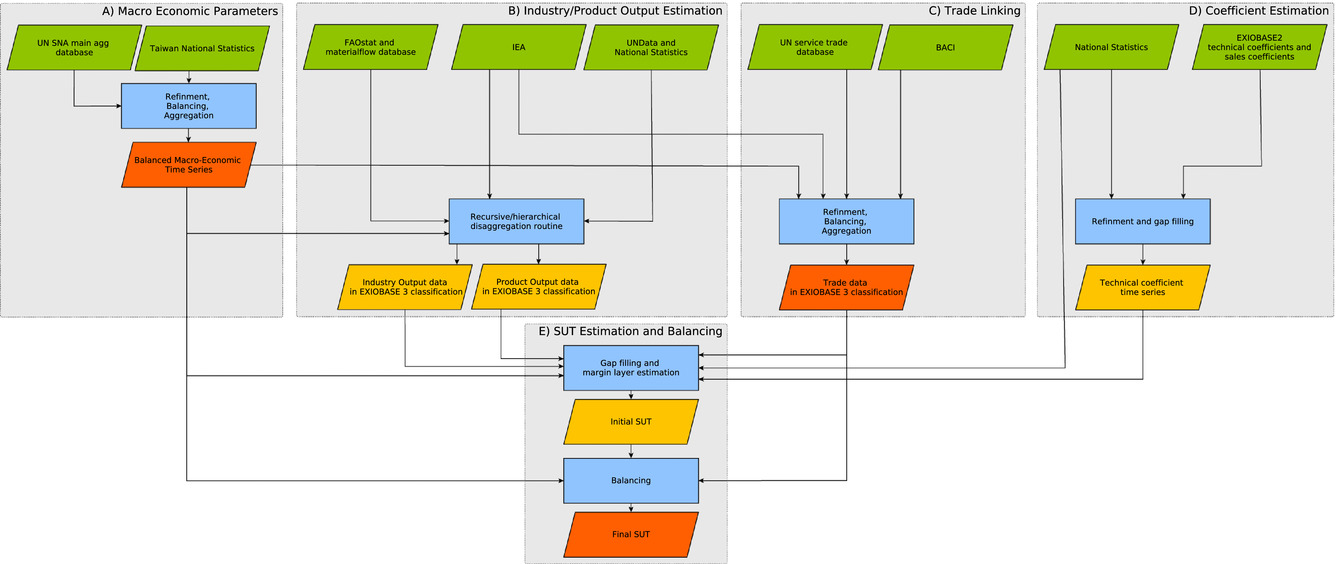
\includegraphics[width=0.5\linewidth]{images/exiobase3} \end{center}

\end{frame}

\begin{frame}{Main Focus of Research}

\begin{enumerate}
\item
  What research has been done on forest or forest landscape embodied
  networks?
\item
  What is the network structure? How can we characterize it?
\item
  What can we say about the potential system dynamics based on network
  structure?
\end{enumerate}

\end{frame}

\begin{frame}{Research: Network Analysis}

\begin{itemize}
\item
  LEMRIO global (Tian 2019)
\item
  LEMRIO local (Chen 2019)
\item
  Your LE-MRIO China
\item
  Your ENA analysis

  \begin{itemize}
  \item
    Small world
  \item
    Modularity
  \item
    Centrality
  \item
    Control
  \item
    Resilience
  \end{itemize}
\end{itemize}

\end{frame}

\begin{frame}{Research: Structural Analysis}

\begin{itemize}
\item
  Analysis = Structure = Robustness
\end{itemize}

\begin{center}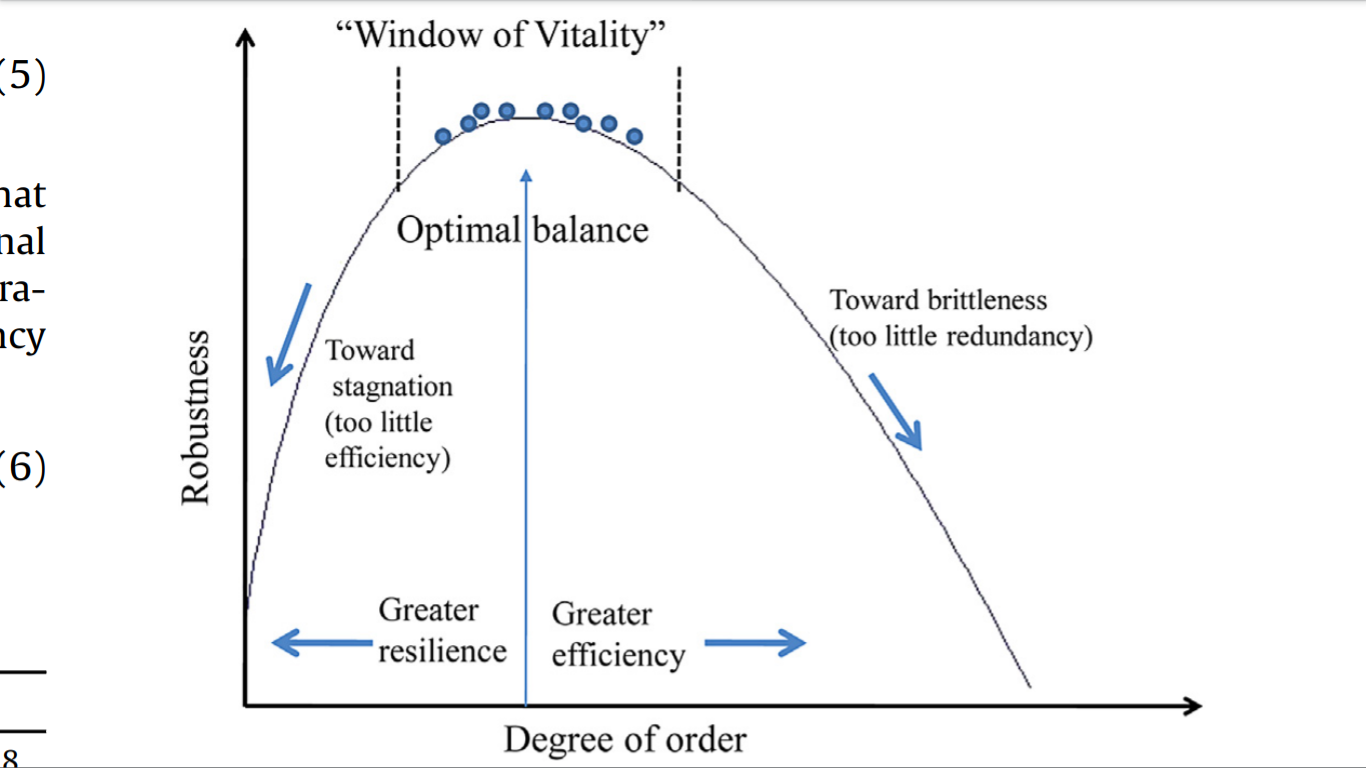
\includegraphics[width=0.5\linewidth]{images/Fath_2015_Fig6} \end{center}

\end{frame}

\begin{frame}{Research: Structural Analysis}

\begin{itemize}
\item
  Overly efficient = Brittle
\item
  Overly redundant = Stagnant
\item
  Both can lead to niche opennings
\item
  Niches can then be filled by natural selection, adaptation or invasion
\end{itemize}

\end{frame}

\begin{frame}{Forest Landscape Networks are More Efficient but Less
Robust}

\begin{center}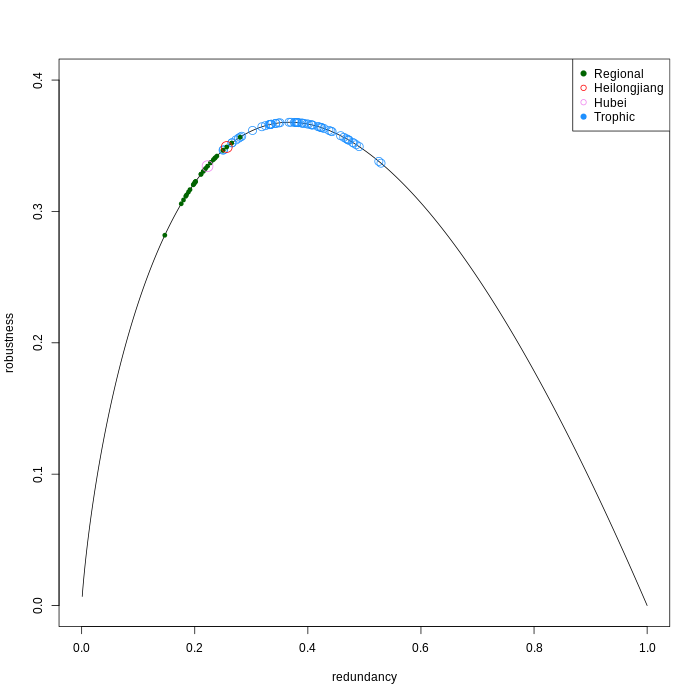
\includegraphics[width=0.5\linewidth]{images/for-rob-red} \end{center}

\end{frame}

\begin{frame}{Caveats}

\begin{itemize}
\item
  Limitations of MRIO
\item
  Potential impacts of storage lags and buffers
\end{itemize}

\end{frame}

\begin{frame}{Future: Next up, climate change variability}

\begin{itemize}
\item
  Next up = Climate change impacts and global scale
\end{itemize}

\begin{center}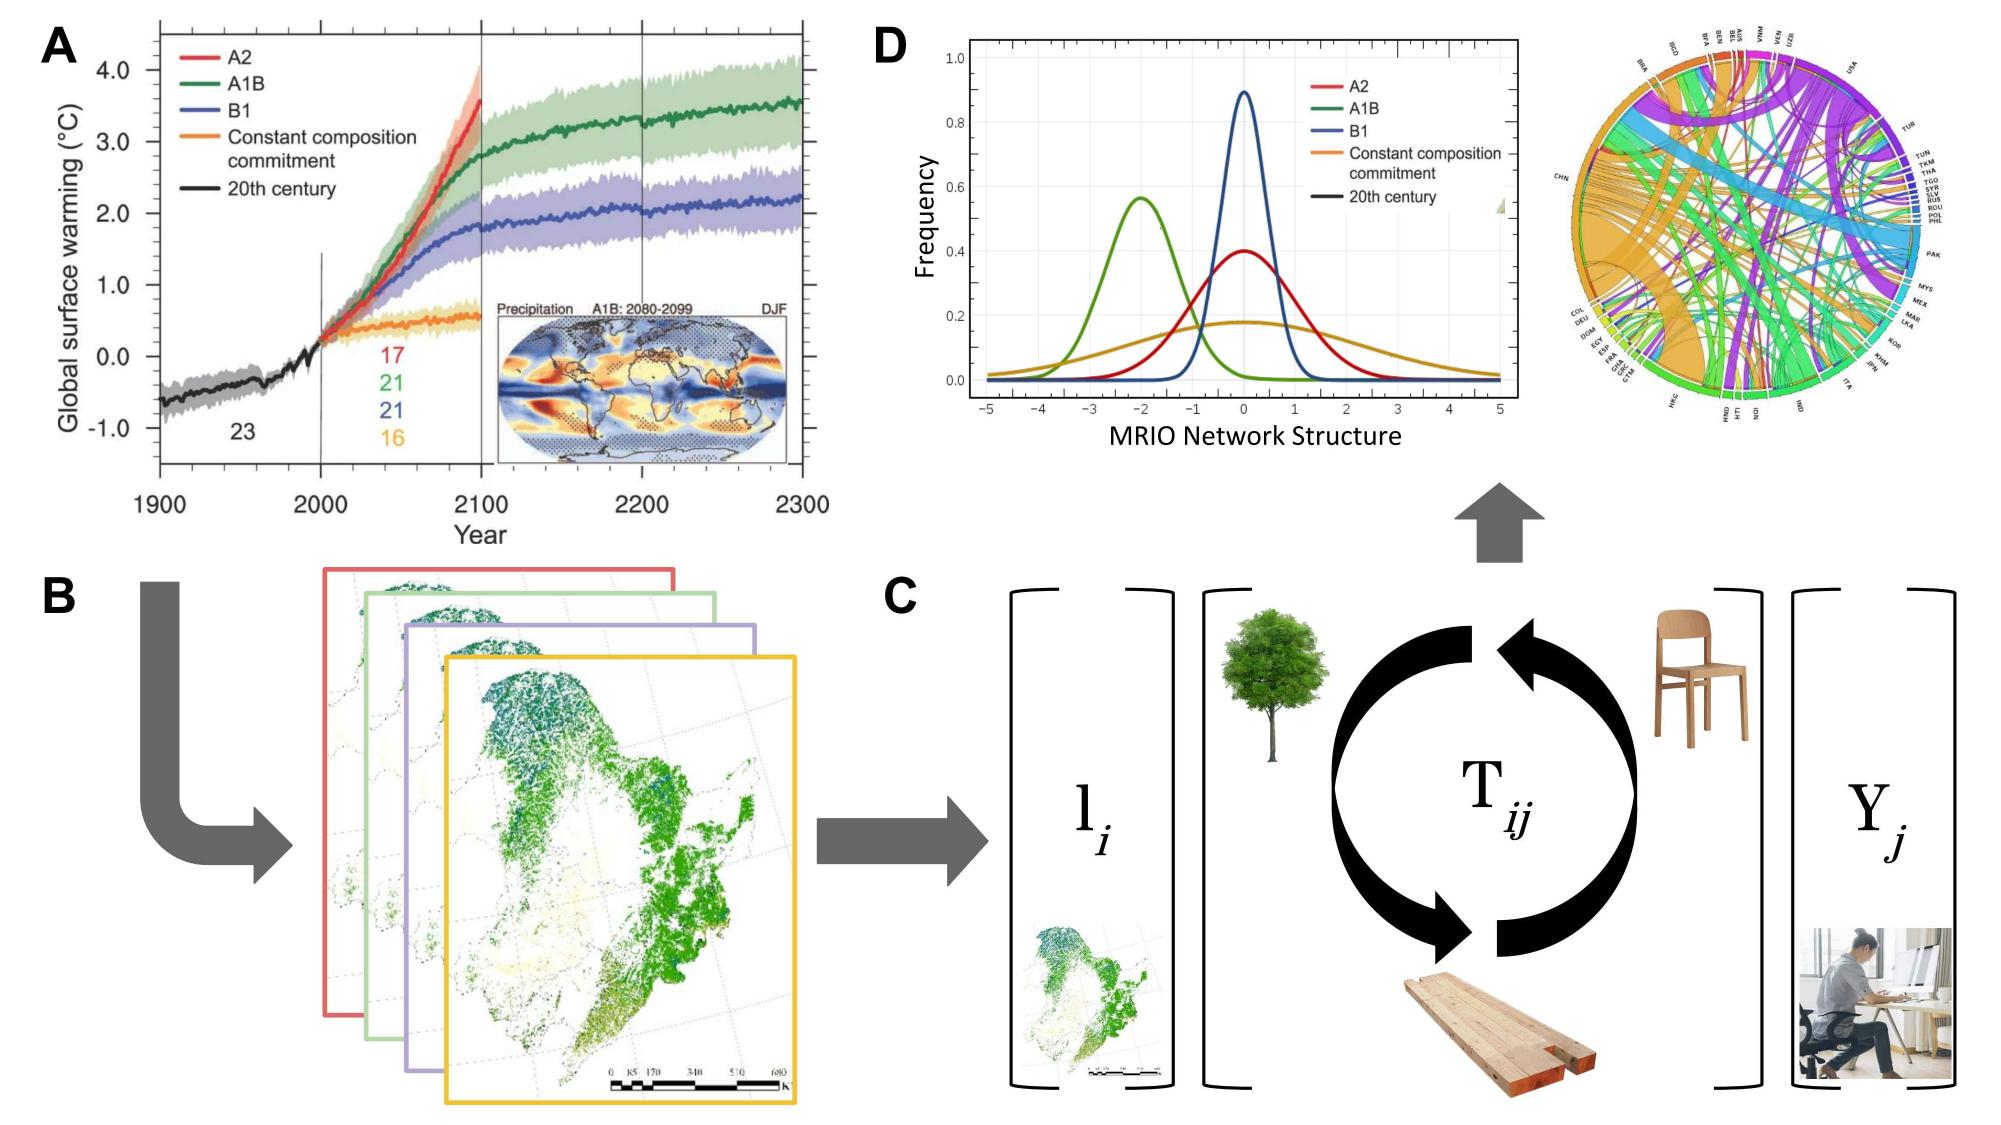
\includegraphics[width=0.5\linewidth]{images/lemrio_climate_change} \end{center}

\end{frame}

\begin{frame}{Future: Next up, climate change variability}

\begin{center}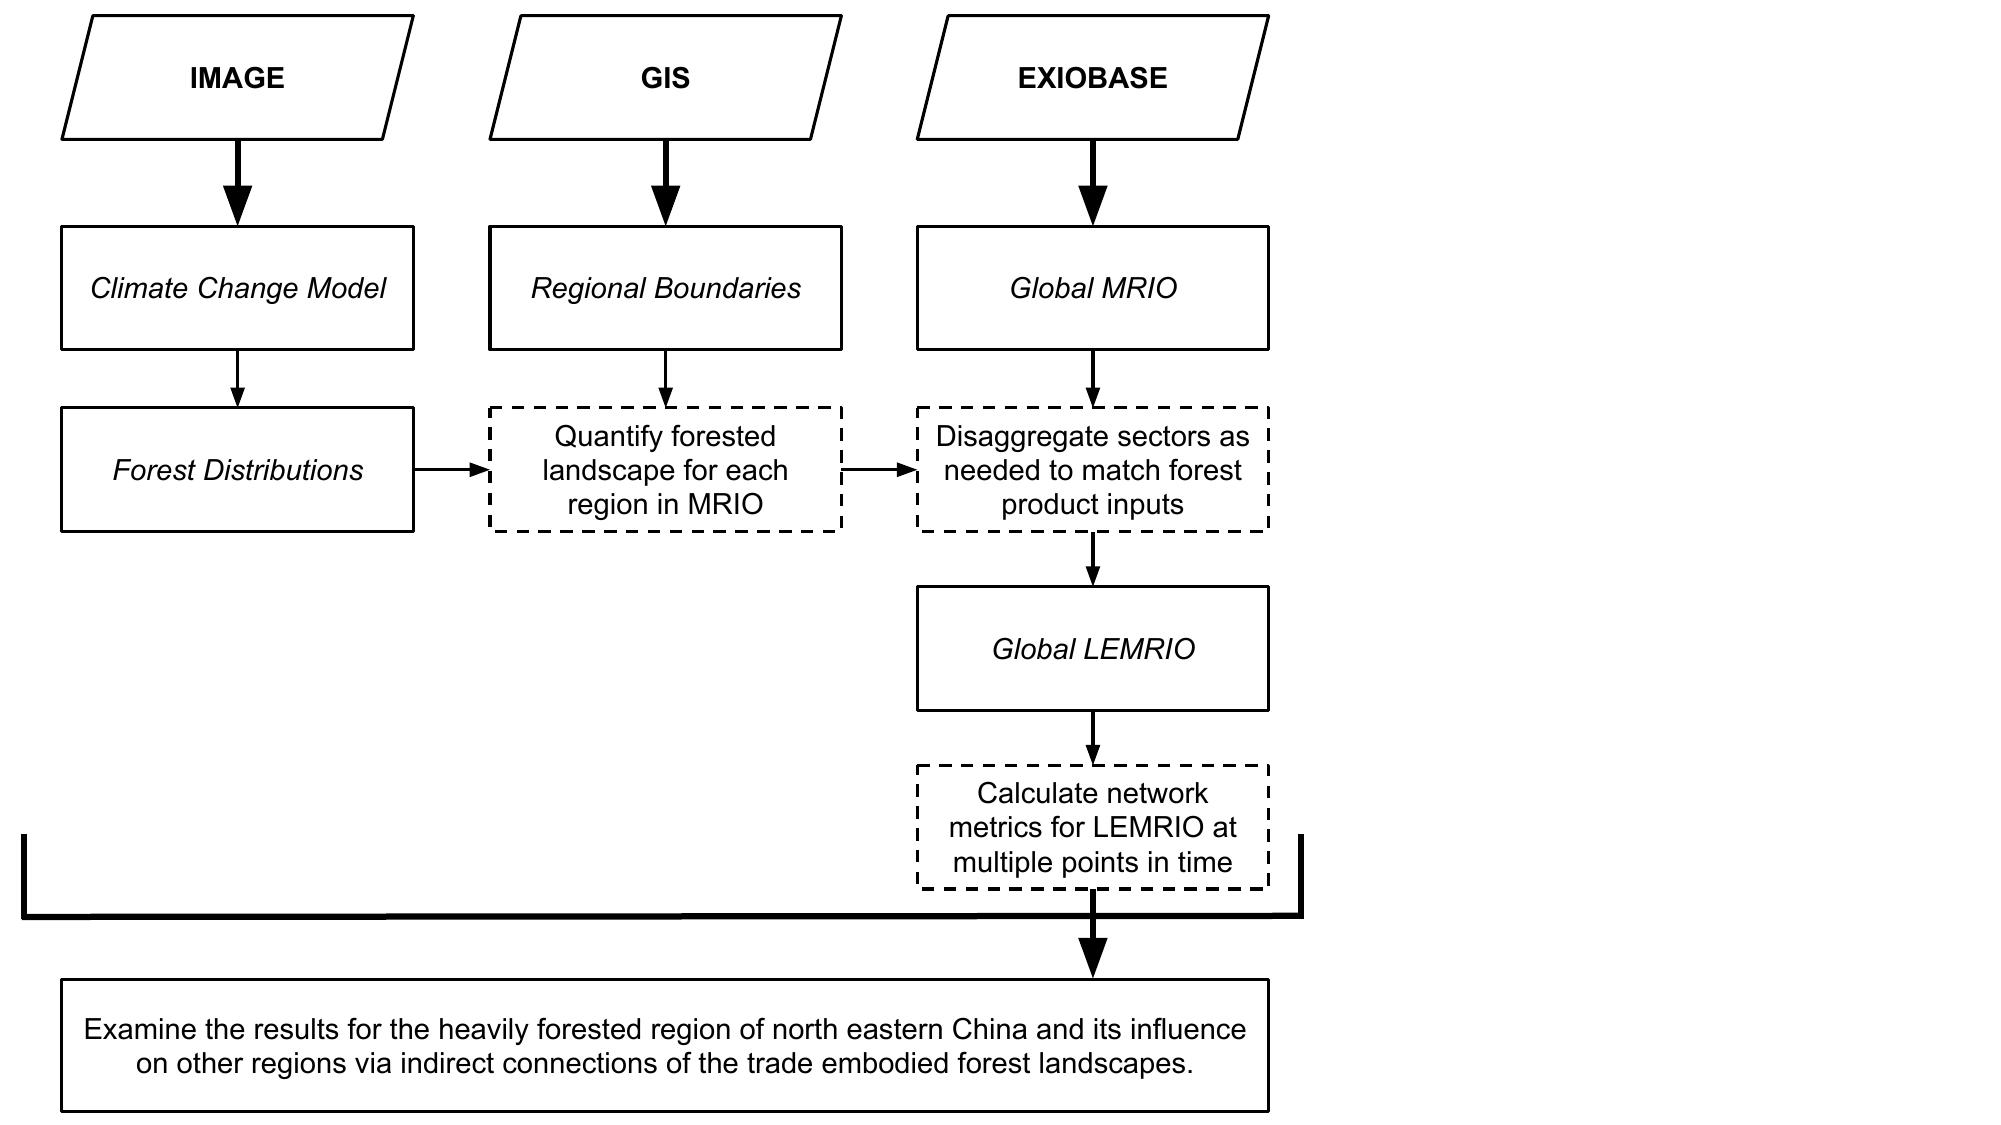
\includegraphics[width=0.1\linewidth]{images/lemrio_climate_workflow} \end{center}

\end{frame}

\begin{frame}{Future Work: Remote Sensing Trade Models}

\begin{center}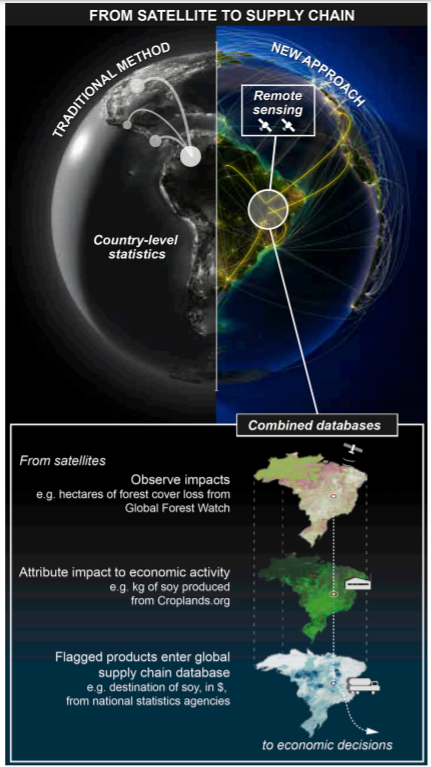
\includegraphics[width=0.1\linewidth]{images/Moran_2020_Fig1} \end{center}

\end{frame}

\begin{frame}{Q \& A}

\end{frame}

\end{document}
